\documentclass[answers]{exam}

%% Language and font encodings
\usepackage{CJKutf8}
\usepackage[english]{babel}
\usepackage[utf8]{inputenc}
\usepackage[T1]{fontenc}
\usepackage{natbib}

%% Color
\usepackage[dvipsnames]{xcolor}

%% Sets page size and margins
\usepackage[a4paper,margin=2cm]{geometry}

%% Useful packages
\usepackage{amsmath}
\usepackage{graphicx}
\usepackage{paralist}
\setlength\FrameSep{4pt}

\begin{document}
\begin{CJK}{UTF8}{min}
\begin{questions}

%%%%%%%%%%%%%%%%%%%%%%%%%
\question[10]{Copy your code comments here.}
\begin{framed}
\begin{compactenum}[A.]
  \item
    Create \texttt{nlayers\_enc} encoding layers using \texttt{add\_link}. There
    are two loops for adding layers because we create one encoder to pass over
    the sentence in order, and one to pass over the sentence in reverse order.
  \item
    The encoding of a sentence is a matrix, each column of which is the
    concatenation of the hidden states of the forward and the backward encoder
    LSTMs at that position. Since both the LSTMs are sized \texttt{n\_units},
    the concatenation of these two hidden states is \texttt{2*n\_units}.
  \item
    The method \texttt{set\_decoder\_state} will feed the encoder output into
    the decoder. The initial implementation takes the cell states and hidden
    state from the final LSTM of the encoder, and feeds them into the first LSTM
    of the decoder.
  \item
    We are performing two encode operations because we are stepping through the
    sentence forwards and backwards at the same time -- see the call to
    \texttt{zip} above -- and we are encoding the `forwards' word using the
    forwards encoder, and the backwards word using the backwards encoder.
  \item
    (\textcolor{red}{TODO add an example.})
    The loss is computed as the cross-entropy over two softmax distributions.
    The cross-entropy is a soft measure of how close the network got to the
    correct answer. Here it is used to find how close the predicted word
    (\texttt{predicted\_out}) was to the expected word
    (\texttt{next\_word\_var}).
  \item
    The \texttt{add\_hook} function adds some code which is to be executed right
    after the computation of the gradient. The \texttt{GradientClipping}
    function will scale gradients down when their L2 norm goes over a certain
    threshold (here 5).
\end{compactenum}
\end{framed}


%%%%%%%%%%%%%%%%%%%%%%%%%
\question[10]{Examine the parallel data and answer questions. (Plots may appear in the appendix.)}
\begin{framed}
\begin{compactenum}[1.]
  \item
    When looking at figures \ref{fig:corr-toks} and \ref{fig:corr-chars}, it
    seems as if English is a more productive language (more `meaning' with fewer
    symbols) when we measure sentence length in tokens, and Japanese is more
    productive when we measure it in characters. There explanations for both
    these observations, which I'll go into in Q3.

    What our graphs do make clear, however, is that there is a linear
    correlation between sentence lengths in English and Japanese. This means
    that we can expect sentence length to change linearly when we translate,
    either as $|f| \approx 1.42|e|$ (tokens) or as $|f| \approx 0.42|e|$
    (characters).
  \item
    In total, there are 97643 and 143581 tokens in the English and Japanese
    data, respectively.
  \item
    There are 7217 and 8246 word types/unique tokens in the English and Japanese
    data, respectively.
  \item
    In the default implementation, the vocabulary size is 3713 for English and
    3949 for Japanese. This means that tokens of 3505 and 4298 token types will
    be replaced with \texttt{\_UNK}, assuming \texttt{\_UNK} is part of the
    vocabulary. These account for 3608 (3.82\%) and 4413 (3.28\%) tokens in the
    data.
  \item
    A vocabulary of 3713 tokens is \emph{really} small. When we look at the most
    common \texttt{\_UNK} words -- \texttt{users protest commerce irony hats} --
    we see that these are still quite common. While $\pm 3.5\%$ does not sound
    like a lot, it will probably cripple a large number of translations with
    \texttt{\_UNK} words. Furthermore, this will probably make \texttt{\_UNK}
    quite difficult for the network to translate, at it will occur in huge
    number of syntactic positions.
    The differences in sentence length seems linear enough not to be a big
    problem.
  \end{compactenum}
\end{framed}


%%%%%%%%%%%%%%%%%%%%%%%%%
\question[10]{What language phenomena might influence what you observed above?}
\begin{framed}
  Our two measures for sentence length seem to contradict one another. Let's
  look at Japanese to see why:
  \begin{compactitem}
  \item {\it High productivity using characters.}
    Japanese uses logograms, and each logogram corresponds to one or more
    syllables. Thus, each character in Japanese can carry far more information
    than in English.
  \item {\it Low productivity using tokens.}
    Japanese also uses post-positional clitics to mark e.g.\ subjects and
    objects~\citep{Hinds-1986}, which are treated as separate tokens.
    Many uses of these clitics, e.g.\ topic, subject, object, are marked in
    English using word order and some vestigial cases, neither of which adds
    tokens.
    Making matters worse, the tokeniser for Japanese seems to treat each
    hiragana as its own token, meaning long and common word endings such as
    `-します' are treated as three separate
    tokens.
  \end{compactitem}
\end{framed}


%%%%%%%%%%%%%%%%%%%%%%%%%
\question[10]{Answers to questions about sampling, beam search, and dynamic programming.}
\begin{framed}
\begin{compactenum}[1.]
\item
  It seems that the argmax version has a bias towards generating more common
  words. For instance, have a look at the translation below:\\
  \begin{tabular}{ll}
    Src & 皮肉 な 笑い を 浮かべ て 彼 は 私 を 見つめ た 。\\
    Ref & he stared at me with a satirical smile .\\
    Hyp & i gave him him he him him him . \_EOS\\
    \multicolumn{2}{l}{%
    The sampling version ``solves'' this problem to the extend that it is a lot less common.
    }\\
    \multicolumn{2}{l}{%
    Unfortunately, this does not mean its translations are better.
    }\\
    Hyp & he gave him from his coming he much . \_EOS\\
    Hyp & i came him him to borrow him him . \_EOS\\
    Hyp & i gave him him for they died job \_EOS
  \end{tabular}
  \item
    First, let's describe a naive version. During decoding I have list of all
    possible next words (i.e.\ the vocabulary) and a score for each next word
    (i.e.\ the log of that word's probability in the network's output
    distribution).
    The naive implementation would simply try each possible word as a next word,
    and recurse, scoring the generated sentences using the sum of the
    log-probabilities. 
    From here, we can add the beam search heuristic, e.g.\ at each step, we only
    keep the $k$ most promising sentences.
  \item
    We cannot implement dynamic programming for this model without changing some
    fundamental parts of the model. The reason for this is that there is no way
    to know when translations are done, or how long the translations will be,
    because we are basically waiting for the \texttt{\_EOS} token to become
    probable (according to the network), and there is no knowing when that will
    happen. 
\end{compactenum}
\end{framed}


%%%%%%%%%%%%%%%%%%%%%%%%%
\question[10]{Experiment with changes to the model, and explain results.}
\begin{framed}
\emph{Your answer here.}
\end{framed}


%%%%%%%%%%%%%%%%%%%%%%%%%
\question[10]{Implement dropout, and explain the results.}
\begin{framed}
\emph{Your answer here.}
\end{framed}


%%%%%%%%%%%%%%%%%%%%%%%%%
\question[20]{Implement attention. This question will be evaluated on the basis of your code.}

\question[10]{Explain the results of implementing attention.}
\begin{framed}
\emph{Your answer here}
\end{framed}

%%%%%%%%%%%%%%%%%%%%%%%%%
\question[10]{Explain what you observe with attention. (Figures may appear in an appendix.)}
\begin{framed}
\emph{Your answer here}
\end{framed}
\end{questions}

\noindent \hrulefill

\clearpage

\bibliography{main}
\bibliographystyle{apalike}

\begin{figure}
  \centering
  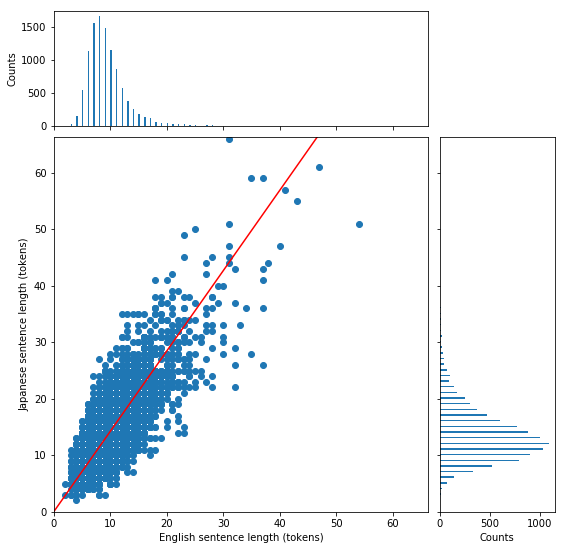
\includegraphics[width=\linewidth]{fig-corr-toks}
  \caption[Sentence lenths (tokens)]%
  {Distribution of and correlation between Japanese and English sentence lengths (tokens)}
  \label{fig:corr-toks}
\end{figure}

\begin{figure}
  \centering
  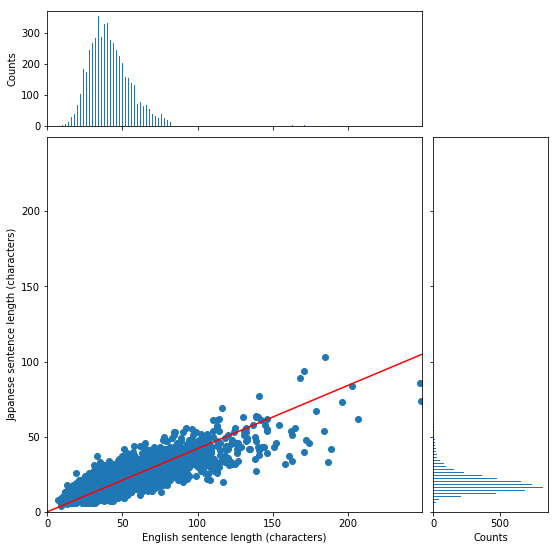
\includegraphics[width=\linewidth]{fig-corr-chars}
  \caption[Sentence lenths (characters)]%
  {Distribution of and correlation between Japanese and English sentence lengths (tokens)}
  \label{fig:corr-chars}
\end{figure}

\begin{figure}
  \centering
  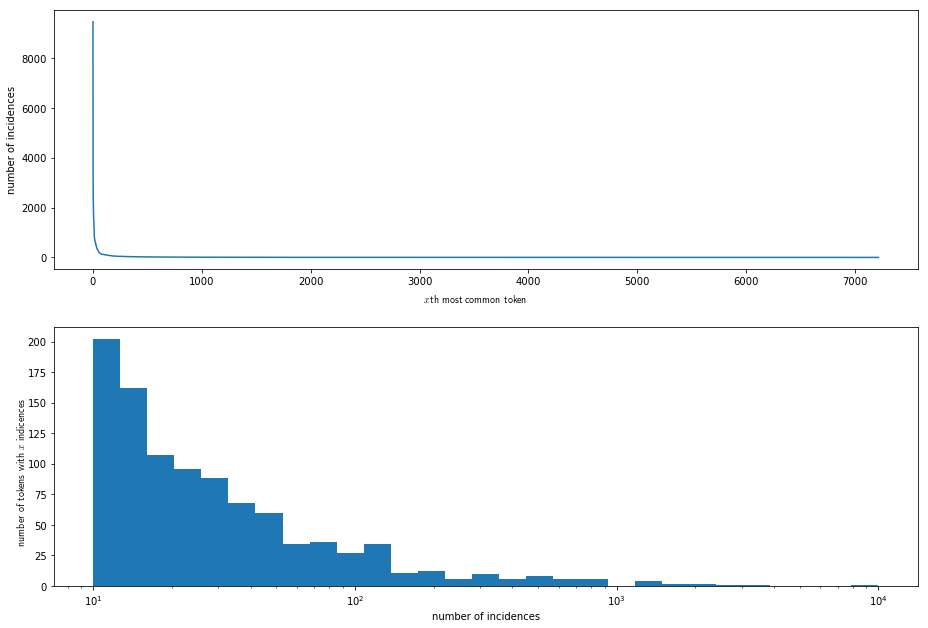
\includegraphics[width=\linewidth]{fig-toks-en}
  \caption{Counts for tokens and token types (English).}
  \label{fig:toks-en}
\end{figure}

\begin{figure}
  \centering
  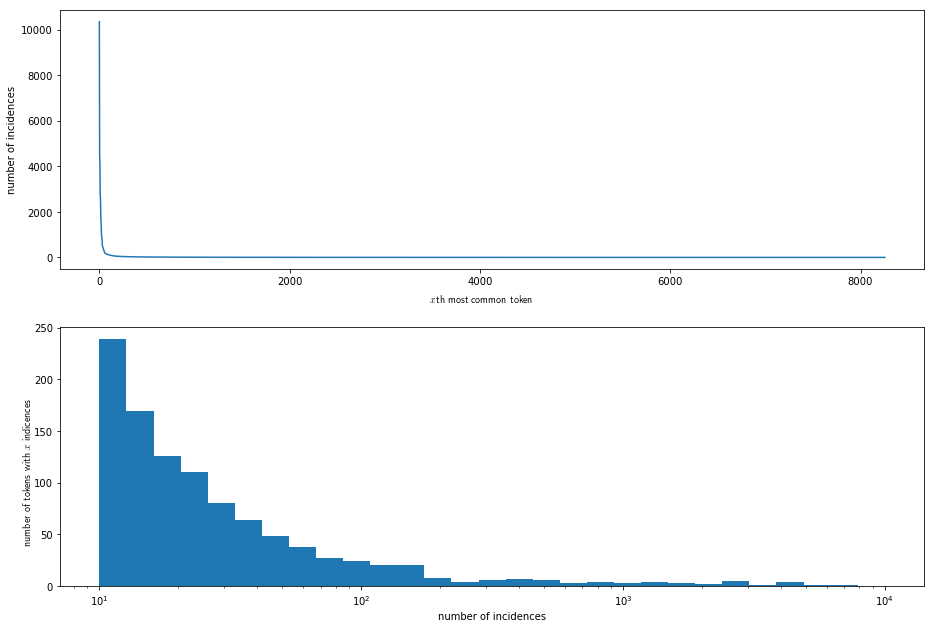
\includegraphics[width=\linewidth]{fig-toks-fr}
  \caption{Counts for tokens and token types (Japanese).}
  \label{fig:toks-fr}
\end{figure}

\end{CJK}
\end{document}